\documentclass[11pt,a4paper]{article}
\usepackage{fontspec}
\setmainfont{TeX Gyre Pagella}
\setsansfont{TeX Gyre Heros}
\setmonofont{DejaVu Sans Mono}[Scale=0.82]
\usepackage{amsmath,amssymb}
\usepackage[margin=2.2cm,top=2cm,bottom=2.2cm]{geometry}
\usepackage{booktabs,array,colortbl}
\usepackage[table]{xcolor}
\usepackage{graphicx}
\usepackage{pdflscape}
\usepackage{enumitem}
\usepackage{titlesec}
\usepackage{fancyhdr}
\usepackage{needspace}
\usepackage{afterpage}
\usepackage[hidelinks]{hyperref}

\definecolor{cinza}{gray}{0.6}
\definecolor{verdeclaro}{HTML}{E8F4EA}
\newcommand{\ok}{\textcolor{green!50!black}{\checkmark}}
\newcommand{\falha}{\textcolor{red}{$\times$}}
\newcommand{\s}[1]{\texttt{#1}}
\newcommand{\q}[1]{$q_{#1}$}

\titleformat{\section}{\sffamily\large\bfseries}{\thesection}{0.6em}{}
\titleformat{\subsection}{\sffamily\normalsize\bfseries}{\thesubsection}{0.6em}{}
\titlespacing*{\section}{0pt}{1.1em}{0.4em}
\setlist{itemsep=1pt,topsep=3pt}
\setlength{\parskip}{5pt}
\setlength{\parindent}{0pt}
\renewcommand{\arraystretch}{1.12}

\pagestyle{fancy}\fancyhf{}
\renewcommand{\headrulewidth}{0.3pt}
\lhead{\small LFA 2026.2 · Trabalho prático}
\rhead{\small Tema 6: E-mail simplificado}
\cfoot{\small\thepage}

%% gerado por gerar_tabelas.py

\newcommand{\TabelaDelta}{%
\begin{tabular}{lccccc}
\toprule
$\delta$ & \texttt{a-z} & \texttt{0-9} & \texttt{.} & \texttt{\_} & \texttt{@} \\
\midrule
$\rightarrow$\,$q_{0}$ & $q_{1}$ & $q_{1}$ & \textcolor{cinza}{$q_p$} & $q_{1}$ & \textcolor{cinza}{$q_p$} \\
$q_{1}$ & $q_{1}$ & $q_{1}$ & $q_{2}$ & $q_{1}$ & $q_{3}$ \\
$q_{2}$ & $q_{1}$ & $q_{1}$ & \textcolor{cinza}{$q_p$} & $q_{1}$ & \textcolor{cinza}{$q_p$} \\
$q_{3}$ & $q_{4}$ & $q_{4}$ & \textcolor{cinza}{$q_p$} & \textcolor{cinza}{$q_p$} & \textcolor{cinza}{$q_p$} \\
$q_{4}$ & $q_{4}$ & $q_{4}$ & $q_{5}$ & \textcolor{cinza}{$q_p$} & \textcolor{cinza}{$q_p$} \\
$q_{5}$ & $q_{6}$ & $q_{9}$ & \textcolor{cinza}{$q_p$} & \textcolor{cinza}{$q_p$} & \textcolor{cinza}{$q_p$} \\
$q_{6}$ & $q_{7}$ & $q_{9}$ & $q_{5}$ & \textcolor{cinza}{$q_p$} & \textcolor{cinza}{$q_p$} \\
\rowcolor{verdeclaro}$*$\,$q_{7}$ & $q_{8}$ & $q_{9}$ & $q_{5}$ & \textcolor{cinza}{$q_p$} & \textcolor{cinza}{$q_p$} \\
\rowcolor{verdeclaro}$*$\,$q_{8}$ & $q_{9}$ & $q_{9}$ & $q_{5}$ & \textcolor{cinza}{$q_p$} & \textcolor{cinza}{$q_p$} \\
$q_{9}$ & $q_{9}$ & $q_{9}$ & $q_{5}$ & \textcolor{cinza}{$q_p$} & \textcolor{cinza}{$q_p$} \\
$q_p$ & \textcolor{cinza}{$q_p$} & \textcolor{cinza}{$q_p$} & \textcolor{cinza}{$q_p$} & \textcolor{cinza}{$q_p$} & \textcolor{cinza}{$q_p$} \\
\bottomrule
\end{tabular}}

\newcommand{\TabelaEstados}{%
\begin{tabular}{@{}l p{0.80\linewidth}@{}}
\toprule
estado & significado \\
\midrule
$q_{0}$ & início, ainda não leu nada \\
$q_{1}$ & no usuário, o último símbolo foi letra, dígito ou \_ (aqui já pode vir o @) \\
$q_{2}$ & no usuário, acabou de ler um ponto (não pode vir ponto nem @) \\
$q_{3}$ & acabou de ler o @, domínio ainda vazio \\
$q_{4}$ & dentro do 1º rótulo do domínio (ainda não leu ponto no domínio) \\
$q_{5}$ & acabou de ler um ponto no domínio, rótulo atual vazio \\
$q_{6}$ & rótulo atual (do 2º em diante) com 1 letra \\
\rowcolor{verdeclaro}$q_{7}$ & rótulo atual com 2 letras, pode ser o último (final) \\
\rowcolor{verdeclaro}$q_{8}$ & rótulo atual com 3 letras, pode ser o último (final) \\
$q_{9}$ & rótulo atual (do 2º em diante) não pode ser o último: tem dígito ou 4 letras ou mais \\
$q_p$ & poço (erro), não sai mais daqui \\
\bottomrule
\end{tabular}}

\newcommand{\TabelaDeltaMinimo}{%
\begin{tabular}{lccccc}
\toprule
$\delta$ & \texttt{a-z} & \texttt{0-9} & \texttt{.} & \texttt{\_} & \texttt{@} \\
\midrule
$\rightarrow$\,$\{q_{0},q_{2}\}$ & $q_{1}$ & $q_{1}$ & \textcolor{cinza}{$q_p$} & $q_{1}$ & \textcolor{cinza}{$q_p$} \\
$q_{1}$ & $q_{1}$ & $q_{1}$ & $\{q_{0},q_{2}\}$ & $q_{1}$ & $q_{3}$ \\
$q_{3}$ & $\{q_{4},q_{9}\}$ & $\{q_{4},q_{9}\}$ & \textcolor{cinza}{$q_p$} & \textcolor{cinza}{$q_p$} & \textcolor{cinza}{$q_p$} \\
$\{q_{4},q_{9}\}$ & $\{q_{4},q_{9}\}$ & $\{q_{4},q_{9}\}$ & $q_{5}$ & \textcolor{cinza}{$q_p$} & \textcolor{cinza}{$q_p$} \\
$q_{5}$ & $q_{6}$ & $\{q_{4},q_{9}\}$ & \textcolor{cinza}{$q_p$} & \textcolor{cinza}{$q_p$} & \textcolor{cinza}{$q_p$} \\
$q_{6}$ & $q_{7}$ & $\{q_{4},q_{9}\}$ & $q_{5}$ & \textcolor{cinza}{$q_p$} & \textcolor{cinza}{$q_p$} \\
\rowcolor{verdeclaro}$*$\,$q_{7}$ & $q_{8}$ & $\{q_{4},q_{9}\}$ & $q_{5}$ & \textcolor{cinza}{$q_p$} & \textcolor{cinza}{$q_p$} \\
\rowcolor{verdeclaro}$*$\,$q_{8}$ & $\{q_{4},q_{9}\}$ & $\{q_{4},q_{9}\}$ & $q_{5}$ & \textcolor{cinza}{$q_p$} & \textcolor{cinza}{$q_p$} \\
$q_p$ & \textcolor{cinza}{$q_p$} & \textcolor{cinza}{$q_p$} & \textcolor{cinza}{$q_p$} & \textcolor{cinza}{$q_p$} & \textcolor{cinza}{$q_p$} \\
\bottomrule
\end{tabular}}

\newcommand{\TabelaMinimizacao}{%
\begin{tabular}{@{}l c l@{}}
\toprule
rodada & blocos & partição \\
\midrule
$P_{0}$ & 2 & {\small $\{q_{0},q_{1},q_{2},q_{3},q_{4},q_{5},q_{6},q_{9},q_p\}$\ $\{q_{7},q_{8}\}$} \\
$P_{1}$ & 4 & {\small $\{q_{0},q_{1},q_{2},q_{3},q_{4},q_{5},q_{9},q_p\}$\ $\{q_{6}\}$\ $\{q_{7}\}$\ $\{q_{8}\}$} \\
$P_{2}$ & 5 & {\small $\{q_{0},q_{1},q_{2},q_{3},q_{4},q_{9},q_p\}$\ $\{q_{5}\}$\ $\{q_{6}\}$\ $\{q_{7}\}$\ $\{q_{8}\}$} \\
$P_{3}$ & 6 & {\small $\{q_{0},q_{1},q_{2},q_{3},q_p\}$\ $\{q_{4},q_{9}\}$\ $\{q_{5}\}$\ $\{q_{6}\}$\ $\{q_{7}\}$\ $\{q_{8}\}$} \\
$P_{4}$ & 7 & {\small $\{q_{0},q_{1},q_{2},q_p\}$\ $\{q_{3}\}$\ $\{q_{4},q_{9}\}$\ $\{q_{5}\}$\ $\{q_{6}\}$\ $\{q_{7}\}$\ $\{q_{8}\}$} \\
$P_{5}$ & 8 & {\small $\{q_{0},q_{2},q_p\}$\ $\{q_{1}\}$\ $\{q_{3}\}$\ $\{q_{4},q_{9}\}$\ $\{q_{5}\}$\ $\{q_{6}\}$\ $\{q_{7}\}$\ $\{q_{8}\}$} \\
$P_{6}$ & 9 & {\small $\{q_{0},q_{2}\}$\ $\{q_{1}\}$\ $\{q_{3}\}$\ $\{q_{4},q_{9}\}$\ $\{q_{5}\}$\ $\{q_{6}\}$\ $\{q_{7}\}$\ $\{q_{8}\}$\ $\{q_p\}$} \\
\bottomrule
\end{tabular}}

\newcommand{\TestesObrig}{%
\begin{tabular}{@{}l l l c >{\raggedright\arraybackslash}p{0.43\linewidth}@{}}
\toprule
palavra & esperado & obtido & ok & para em / motivo \\
\midrule
\texttt{aluno@uni.edu.br} & aceita & aceita & \ok & {\scriptsize termina em $q_{7}$} \\
\texttt{joao.silva\_2@mail.com} & aceita & aceita & \ok & {\scriptsize termina em $q_{8}$} \\
\texttt{j@a.io} & aceita & aceita & \ok & {\scriptsize termina em $q_{7}$} \\
\texttt{.joao@mail.com} & rejeita & rejeita & \ok & {\scriptsize $q_p$, pos.\,1: o usuário não pode começar com ponto} \\
\texttt{joao..silva@mail.com} & rejeita & rejeita & \ok & {\scriptsize $q_p$, pos.\,6: o usuário não pode ter dois pontos seguidos} \\
\texttt{joao@mail} & rejeita & rejeita & \ok & {\scriptsize $q_{4}$: o domínio precisa ter pelo menos dois rótulos separados por ponto} \\
\texttt{joao@@mail.com} & rejeita & rejeita & \ok & {\scriptsize $q_p$, pos.\,6: o e-mail tem que ter exatamente um @} \\
\texttt{joao@mail.c} & rejeita & rejeita & \ok & {\scriptsize $q_{6}$: o último rótulo tem só 1 letra (precisa de 2 ou 3)} \\
\texttt{joao@mail.com1} & rejeita & rejeita & \ok & {\scriptsize $q_{9}$: o último rótulo precisa ter só letras, 2 ou 3} \\
\bottomrule
\end{tabular}}
\newcommand{\TestesObrigTotal}{9/9}

\newcommand{\TestesProprias}{%
\begin{tabular}{@{}l l l c >{\raggedright\arraybackslash}p{0.43\linewidth}@{}}
\toprule
palavra & esperado & obtido & ok & para em / motivo \\
\midrule
\texttt{a@b.cc} & aceita & aceita & \ok & {\scriptsize termina em $q_{7}$} \\
\texttt{a@b.ccc} & aceita & aceita & \ok & {\scriptsize termina em $q_{8}$} \\
\texttt{\_@b.cc} & aceita & aceita & \ok & {\scriptsize termina em $q_{7}$} \\
\texttt{1@2.br} & aceita & aceita & \ok & {\scriptsize termina em $q_{7}$} \\
\texttt{joao\_@mail.com} & aceita & aceita & \ok & {\scriptsize termina em $q_{8}$} \\
\texttt{\_joao@mail.com} & aceita & aceita & \ok & {\scriptsize termina em $q_{8}$} \\
\texttt{a.b.c.d@mail.com} & aceita & aceita & \ok & {\scriptsize termina em $q_{8}$} \\
\texttt{joao@123.456.com} & aceita & aceita & \ok & {\scriptsize termina em $q_{8}$} \\
\texttt{joao@a.b.c.de} & aceita & aceita & \ok & {\scriptsize termina em $q_{7}$} \\
\texttt{joao@mail.comp.br} & aceita & aceita & \ok & {\scriptsize termina em $q_{7}$} \\
\texttt{joao@x1.y2.org} & aceita & aceita & \ok & {\scriptsize termina em $q_{8}$} \\
\texttt{joao@mail.co.uk} & aceita & aceita & \ok & {\scriptsize termina em $q_{7}$} \\
\texttt{user\_\_name@site.net} & aceita & aceita & \ok & {\scriptsize termina em $q_{8}$} \\
\texttt{z9.y\_8@q.zz} & aceita & aceita & \ok & {\scriptsize termina em $q_{7}$} \\
\texttt{nome.sobrenome@sub.dominio.gov.br} & aceita & aceita & \ok & {\scriptsize termina em $q_{7}$} \\
$\varepsilon$ (vazia) & rejeita & rejeita & \ok & {\scriptsize $q_{0}$: palavra vazia} \\
\texttt{a@b.c} & rejeita & rejeita & \ok & {\scriptsize $q_{6}$: o último rótulo tem só 1 letra (precisa de 2 ou 3)} \\
\texttt{a@b.cccc} & rejeita & rejeita & \ok & {\scriptsize $q_{9}$: o último rótulo precisa ter só letras, 2 ou 3} \\
\texttt{joao} & rejeita & rejeita & \ok & {\scriptsize $q_{1}$: falta o @ e o domínio} \\
\texttt{joao.} & rejeita & rejeita & \ok & {\scriptsize $q_{2}$: falta o @ e o domínio, e o usuário não pode terminar com ponto} \\
\texttt{@mail.com} & rejeita & rejeita & \ok & {\scriptsize $q_p$, pos.\,1: o usuário não pode ser vazio} \\
\texttt{joao@} & rejeita & rejeita & \ok & {\scriptsize $q_{3}$: domínio vazio} \\
\texttt{joao.@mail.com} & rejeita & rejeita & \ok & {\scriptsize $q_p$, pos.\,6: o usuário não pode terminar com ponto} \\
\texttt{joao@.mail.com} & rejeita & rejeita & \ok & {\scriptsize $q_p$, pos.\,6: o domínio não pode começar com ponto} \\
\texttt{joao@mail..com} & rejeita & rejeita & \ok & {\scriptsize $q_p$, pos.\,11: dois pontos seguidos no domínio (rótulo vazio)} \\
\texttt{joao@mail.com.} & rejeita & rejeita & \ok & {\scriptsize $q_{5}$: não pode terminar com ponto (último rótulo vazio)} \\
\texttt{joao@mail.c0m} & rejeita & rejeita & \ok & {\scriptsize $q_{9}$: o último rótulo precisa ter só letras, 2 ou 3} \\
\texttt{joao@mail\_x.com} & rejeita & rejeita & \ok & {\scriptsize $q_p$, pos.\,10: não pode ter \_ no domínio} \\
\texttt{joao@mail.com@x.com} & rejeita & rejeita & \ok & {\scriptsize $q_p$, pos.\,14: o e-mail tem que ter exatamente um @} \\
\texttt{joao@mailcom} & rejeita & rejeita & \ok & {\scriptsize $q_{4}$: o domínio precisa ter pelo menos dois rótulos separados por ponto} \\
\texttt{Joao@mail.com} & rejeita & rejeita & \ok & {\scriptsize $q_p$, pos.\,1: o símbolo 'J' não está no alfabeto} \\
\texttt{joão@mail.com} & rejeita & rejeita & \ok & {\scriptsize $q_p$, pos.\,3: o símbolo 'ã' não está no alfabeto} \\
\texttt{joao␣silva@mail.com} & rejeita & rejeita & \ok & {\scriptsize $q_p$, pos.\,5: o símbolo ' ' não está no alfabeto} \\
\texttt{joao@mail-x.com} & rejeita & rejeita & \ok & {\scriptsize $q_p$, pos.\,10: o símbolo '-' não está no alfabeto} \\
\texttt{joao@mail.com␣} & rejeita & rejeita & \ok & {\scriptsize $q_p$, pos.\,14: o símbolo ' ' não está no alfabeto} \\
\texttt{.} & rejeita & rejeita & \ok & {\scriptsize $q_p$, pos.\,1: o usuário não pode começar com ponto} \\
\texttt{@} & rejeita & rejeita & \ok & {\scriptsize $q_p$, pos.\,1: o usuário não pode ser vazio} \\
\bottomrule
\end{tabular}}
\newcommand{\TestesPropriasTotal}{37/37}

\newcommand{\TestesHifen}{%
\begin{tabular}{@{}l l l c >{\raggedright\arraybackslash}p{0.43\linewidth}@{}}
\toprule
palavra & esperado & obtido & ok & para em / motivo \\
\midrule
\texttt{joao@mail-x.com} & aceita & aceita & \ok & {\scriptsize termina em $q_{8}$} \\
\texttt{joao@a-b-c.com.br} & aceita & aceita & \ok & {\scriptsize termina em $q_{7}$} \\
\texttt{joao@a--b.com} & aceita & aceita & \ok & {\scriptsize termina em $q_{8}$} \\
\texttt{joao@uni.sub-dom.br} & aceita & aceita & \ok & {\scriptsize termina em $q_{7}$} \\
\texttt{aluno@uni.edu.br} & aceita & aceita & \ok & {\scriptsize termina em $q_{7}$} \\
\texttt{j@a.io} & aceita & aceita & \ok & {\scriptsize termina em $q_{7}$} \\
\texttt{joao@-mail.com} & rejeita & rejeita & \ok & {\scriptsize $q_p$, pos.\,6: rótulo do domínio não pode começar com hífen} \\
\texttt{joao@mail-.com} & rejeita & rejeita & \ok & {\scriptsize $q_p$, pos.\,11: rótulo do domínio não pode terminar com hífen} \\
\texttt{joao@mail.-com} & rejeita & rejeita & \ok & {\scriptsize $q_p$, pos.\,11: rótulo do domínio não pode começar com hífen} \\
\texttt{joao@mail.com-} & rejeita & rejeita & \ok & {\scriptsize $q_{11}$: rótulo do domínio não pode terminar com hífen} \\
\texttt{joao@mail.co-m} & rejeita & rejeita & \ok & {\scriptsize $q_{9}$: o último rótulo precisa ter só letras, 2 ou 3} \\
\texttt{jo-ao@mail.com} & rejeita & rejeita & \ok & {\scriptsize $q_p$, pos.\,3: hífen só é permitido no domínio} \\
\texttt{joao@mail} & rejeita & rejeita & \ok & {\scriptsize $q_{4}$: o domínio precisa ter pelo menos dois rótulos separados por ponto} \\
\texttt{joao@mail.com1} & rejeita & rejeita & \ok & {\scriptsize $q_{9}$: o último rótulo precisa ter só letras, 2 ou 3} \\
\bottomrule
\end{tabular}}
\newcommand{\TestesHifenTotal}{14/14}

\newcommand{\TestesTotal}{60/60}


\begin{document}

\begin{center}
{\small Linguagens Formais e Autômatos · Ciência da Computação · 2026.2}\\[2pt]
{\small Prof. Dr. Leonardo Angelo}\\[10pt]
{\sffamily\LARGE\bfseries Tema 6: E-mail simplificado (AFD)}\\[10pt]
Alawander \quad·\quad Bernardo Barcellos Leite \quad·\quad Dereck \quad·\quad Pietro Santana \quad·\quad Roberto Vieira
\end{center}
\vspace{4pt}

\section{O problema}

O tema é validar e-mails de um cadastro usando regras simplificadas. A palavra de entrada é o
e-mail inteiro, e o autômato lê um símbolo por vez até decidir se aceita ou rejeita.

O alfabeto é
\[
\Sigma = \{\s{a},\dots,\s{z}\} \cup \{\s{0},\dots,\s{9}\} \cup \{\s{.},\ \s{\_},\ \s{@}\},
\]
com 26 letras, 10 dígitos e 3 símbolos, ou seja, $|\Sigma| = 39$. Letras maiúsculas, acentos,
espaço e hífen não fazem parte de $\Sigma$.

A regra da linguagem, do jeito que nós entendemos: o e-mail tem a forma \s{usuário@domínio}, com um
único \s{@}. O usuário é uma sequência não vazia de letras, dígitos, pontos e \s{\_}, onde o ponto
não pode aparecer no começo, no fim nem duas vezes seguidas. O domínio é formado por dois ou mais
rótulos separados por ponto; cada rótulo tem pelo menos um símbolo e só usa letras e dígitos. O último
rótulo é diferente dos outros: ele só pode ter letras, e tem que ter 2 ou 3.

Por exemplo, \s{aluno@uni.edu.br} e \s{j@a.io} estão na linguagem, enquanto \s{joao@mail} (um rótulo só),
\s{joao@mail.c} (último rótulo com uma letra) e \s{.joao@mail.com} não estão. A menor palavra aceita tem
6 símbolos, como \s{a@b.cc}.

\section{Modelagem}

Para montar os estados, pensamos no que o autômato precisa guardar sobre o que já foi lido para
conseguir decidir o resto. Chegamos em quatro coisas:

\begin{enumerate}
  \item se ele está lendo o usuário ou o domínio (o \s{@} faz essa troca e só pode aparecer uma vez);
  \item no usuário, se o último símbolo foi um ponto. Com isso dá para barrar \s{..}, ponto logo antes do
        \s{@} e ponto no começo;
  \item no domínio, se já apareceu algum ponto. Enquanto não aparece, estamos no primeiro rótulo, e o
        primeiro rótulo nunca pode ser o último, porque o domínio precisa de pelo menos dois;
  \item quantas letras tem o rótulo atual. Basta contar até 3: depois de um dígito ou da quarta letra o
        rótulo não pode mais ser o último, e aí não importa mais o tamanho dele.
\end{enumerate}

Com isso ficamos com os estados da Tabela~1. As linhas em verde são os estados finais.

\begin{table}[htbp]
\centering\small\TabelaEstados\\[3pt]
{\small Tabela 1: estados do AFD e o que cada um significa.}
\end{table}

Alguns pontos da modelagem:
\begin{itemize}
  \item Só \q7 e \q8 são finais. Para chegar neles é preciso ter passado por um ponto do domínio (então
        há pelo menos dois rótulos) e o rótulo atual precisa ter exatamente 2 ou 3 letras.
  \item O autômato não precisa saber de antemão qual rótulo vai ser o último. Em \q7, por exemplo, se a
        palavra acabar ali o rótulo era o último; se vier um ponto, ele era um rótulo do meio e voltamos
        para \q5. O mesmo estado serve para os dois casos.
  \item Os estados \q0 e \q2 têm as mesmas transições: nos dois não pode vir ponto nem \s{@}. Mesmo assim
        deixamos separados, porque \q0 é ``não li nada'' e \q2 é ``acabei de ler um ponto''. O mesmo acontece
        com \q4 e \q9 (ver Seção 6).
  \item O poço $q_p$ aparece na tabela e no código. Ele recebe toda transição inválida e também qualquer
        símbolo fora de $\Sigma$, e não tem saída.
\end{itemize}

\section{Definição formal}

$M = (Q, \Sigma, \delta, q_0, F)$, onde
\begin{itemize}
  \item $Q = \{q_0, q_1, q_2, q_3, q_4, q_5, q_6, q_7, q_8, q_9, q_p\}$ (11 estados);
  \item $\Sigma$ é o alfabeto da Seção 1;
  \item $q_0$ é o estado inicial;
  \item $F = \{q_7, q_8\}$;
  \item $\delta : Q \times \Sigma \to Q$ é dada pela Tabela~2.
\end{itemize}

Na tabela, a coluna \s{a-z} vale para cada uma das 26 letras e a coluna \s{0-9} para cada um dos 10 dígitos,
porque todas as letras levam ao mesmo estado (e todos os dígitos também) em qualquer linha. Escrita
símbolo por símbolo, seriam $11 \times 39 = 429$ células, todas preenchidas. No código
(\s{src/email\_afd.py}) a tabela está escrita do mesmo jeito, por grupos, e o programa expande cada grupo
para os símbolos e confere se nenhuma das 429 células ficou sem definir.

\begin{table}[htbp]
\centering\TabelaDelta\\[4pt]
{\small Tabela 2: função de transição. $\rightarrow$ estado inicial, $*$ estado final;
para qualquer símbolo $x \notin \Sigma$, $\delta(q, x) = q_p$.}
\end{table}

\section{Diagrama}

O diagrama está na página deitada a seguir e também em \s{docs/diagrama.png}. Os estados finais são os de círculo duplo. Ele foi gerado pelo próprio programa
a partir da tabela $\delta$ (opção \s{--dot}) e desenhado com o Graphviz, então o desenho é igual ao código.
Para o diagrama não ficar poluído, as setas que vão para o poço não aparecem. A versão com todas as setas
para o poço está em \s{docs/diagrama\_com\_poco.png}.

\afterpage{%
\begin{landscape}
\thispagestyle{empty}
\begin{center}
{\sffamily\bfseries Diagrama do AFD}\\[6pt]
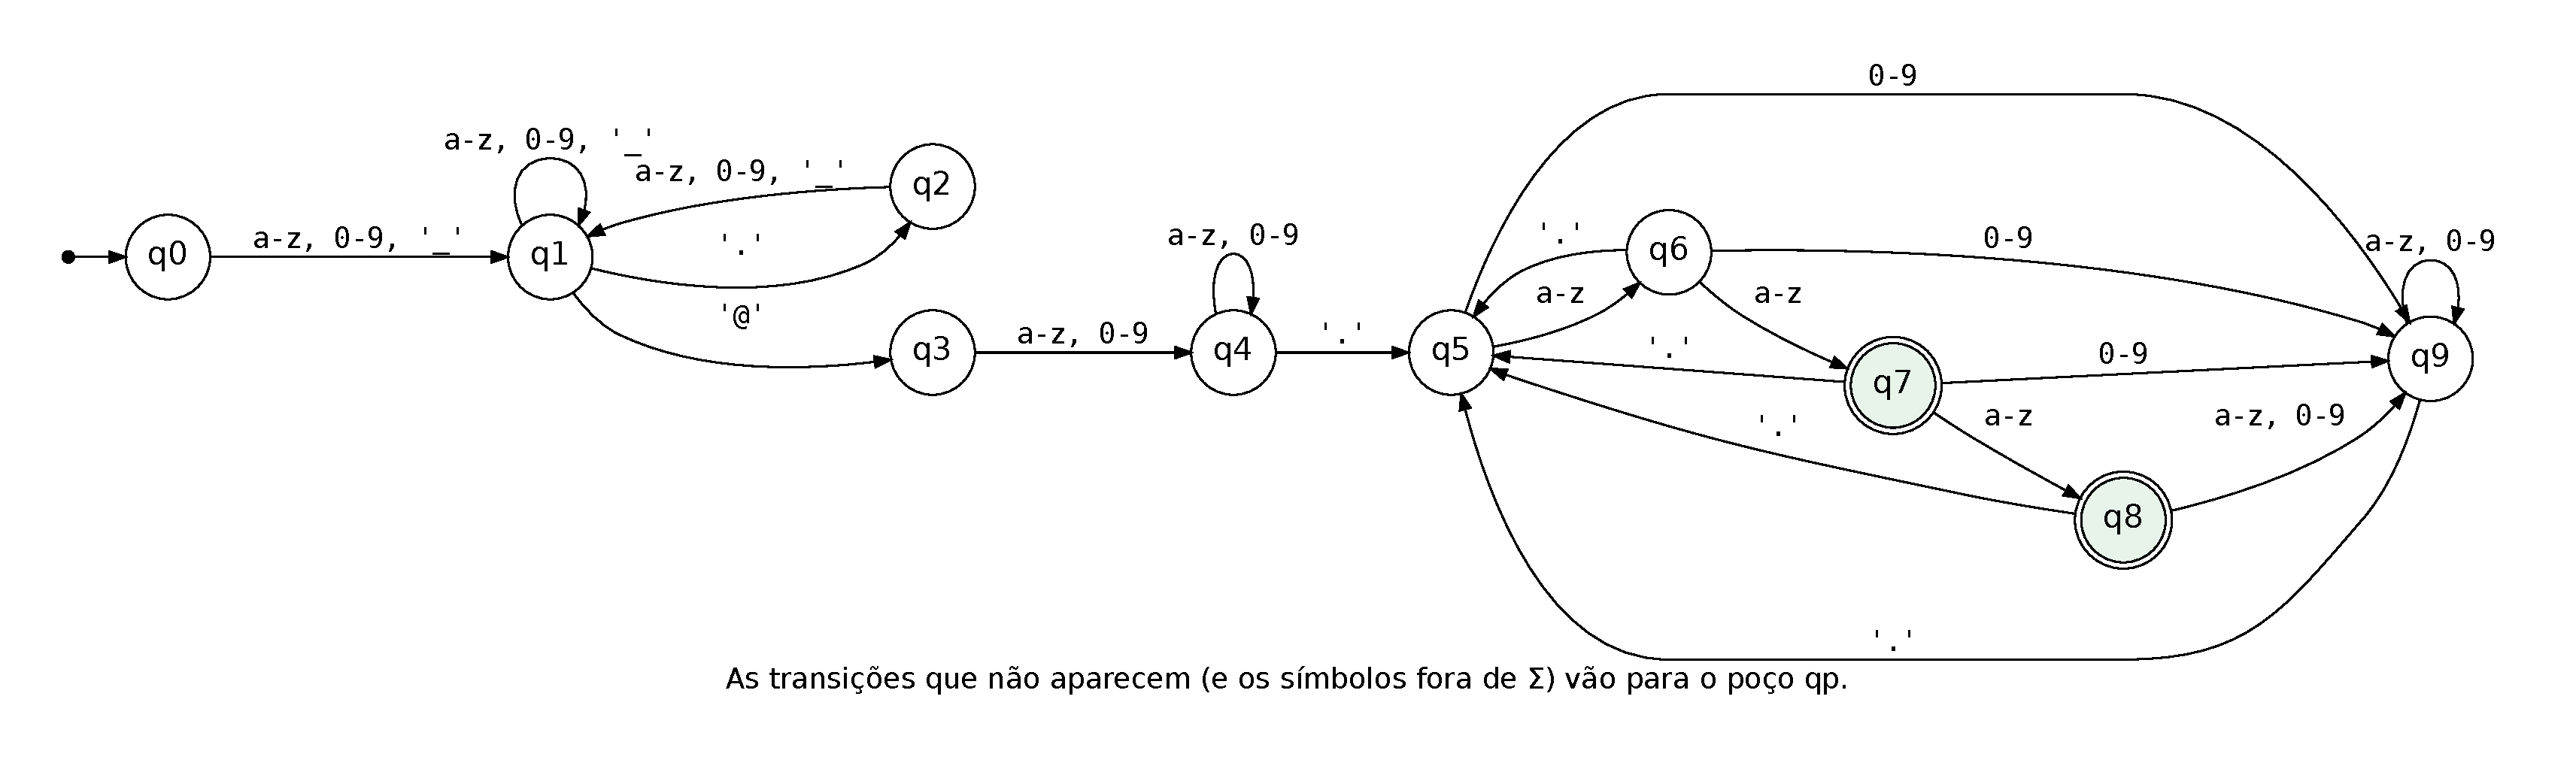
\includegraphics[width=\linewidth,height=6.3cm,keepaspectratio]{diagrama.pdf}\\[10pt]
{\sffamily\bfseries Versão com hífen (Seção 6.5)}\\[6pt]
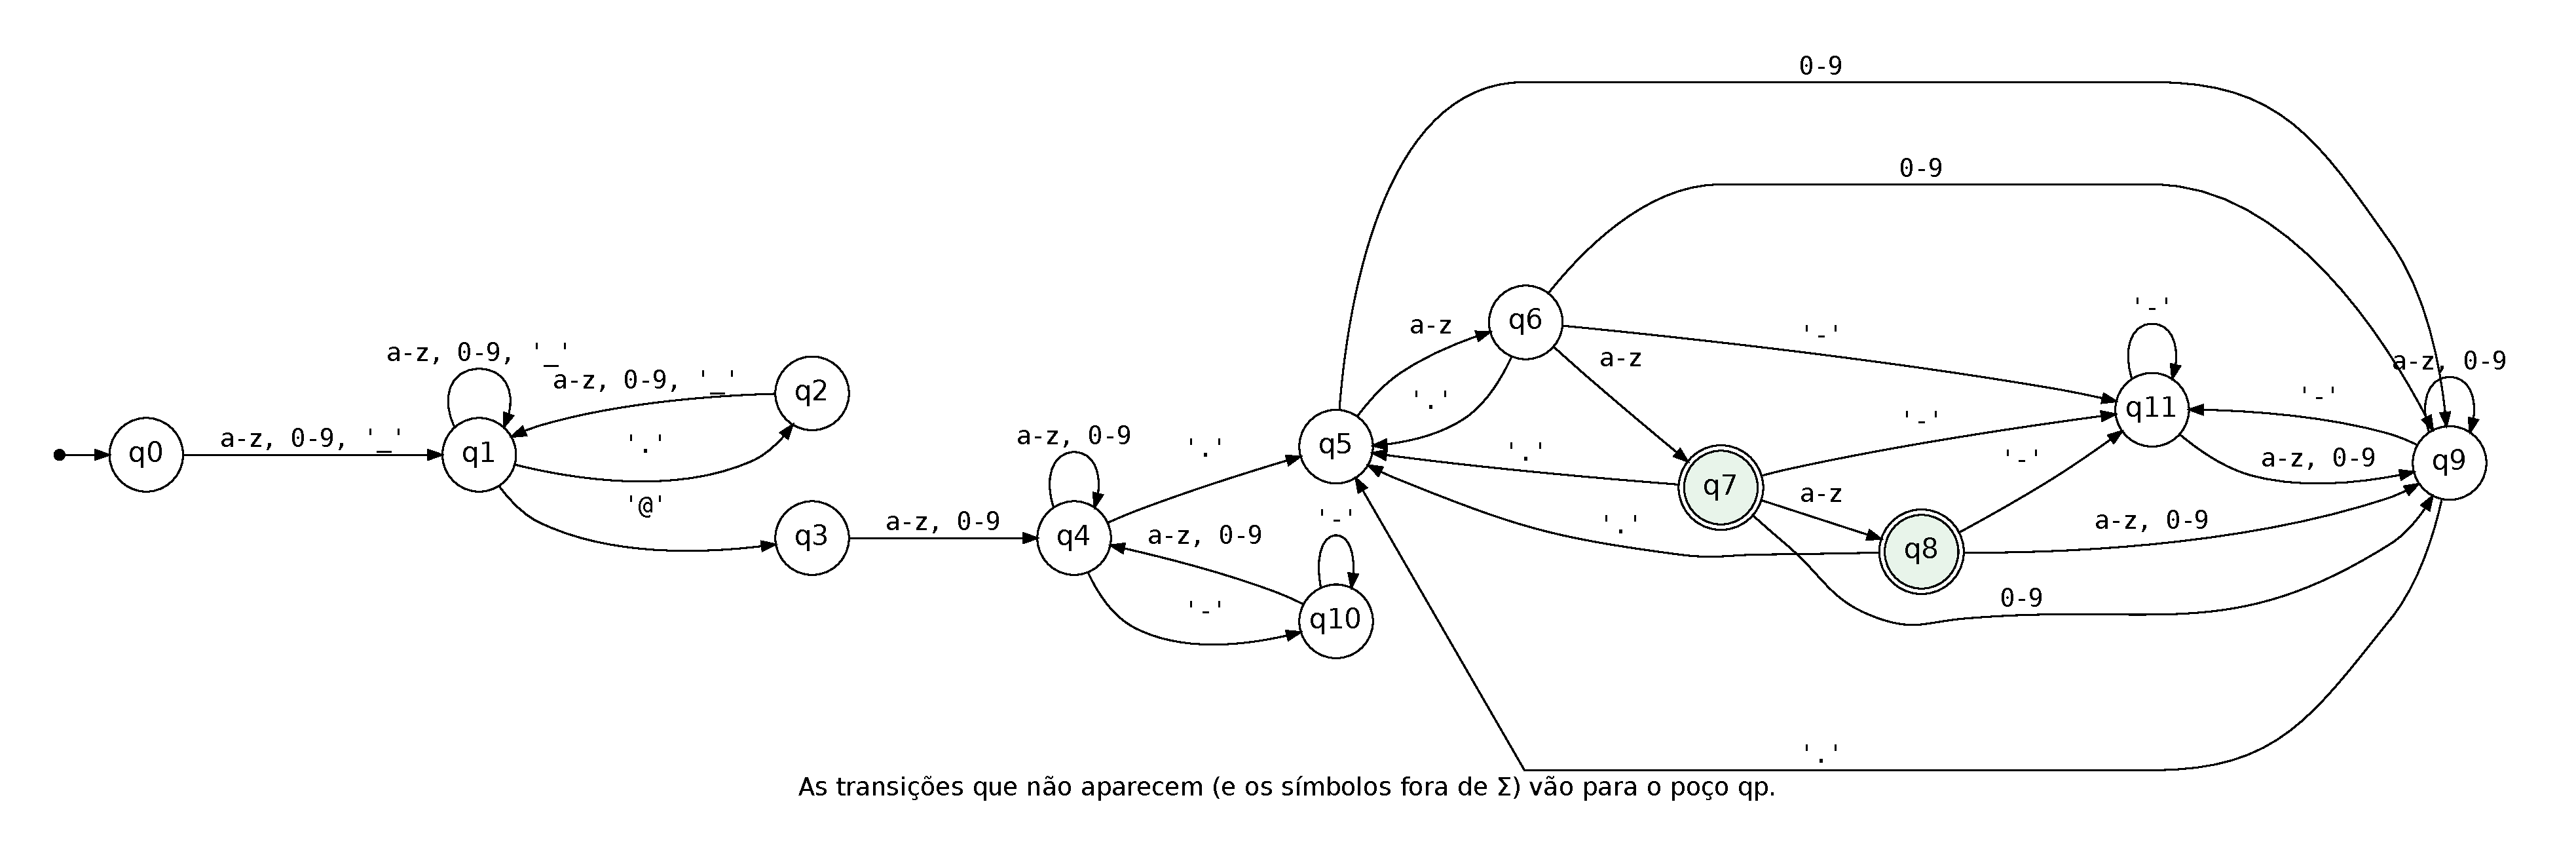
\includegraphics[width=\linewidth,height=7.2cm,keepaspectratio]{diagrama_hifen.pdf}
\end{center}
\end{landscape}}

\section{Testes}

Os testes ficam na pasta \s{testes/}, em arquivos de texto com o resultado esperado de cada palavra. O script
\s{testes/rodar\_testes.py} roda todos e mostra, para cada palavra, o esperado, o obtido e se bateu.
Resultado: \TestesTotal{} testes passando (\TestesObrigTotal{} obrigatórias, \TestesPropriasTotal{} nossas
e \TestesHifenTotal{} da versão com hífen).

\subsection*{Palavras obrigatórias}
\begin{center}\footnotesize\TestesObrig\end{center}

\subsection*{Palavras do grupo}
Escolhemos 15 palavras aceitas e 22 rejeitadas tentando pegar as bordas: a menor palavra aceita
(\s{a@b.cc}), uma com um símbolo a menos (\s{a@b.c}) e uma com um a mais (\s{a@b.cccc}), a palavra vazia, o
ponto em cada posição proibida e cada tipo de símbolo fora de $\Sigma$ (maiúscula, acento, espaço e hífen).
Também colocamos palavras que passam por todos os estados.
\begin{center}\footnotesize\TestesProprias\end{center}

Além disso, fizemos um teste a mais (\s{testes/verificacao\_exaustiva.py}): escrevemos as regras do enunciado
de outro jeito, sem autômato, só com \s{if} e fatiamento de string, e comparamos com o AFD. Testamos todas as
335\,923 palavras de tamanho 0 a 7 formadas por \s{a}, \s{1}, \s{.}, \s{\_}, \s{@} e \s{A} (o \s{A} faz o papel
de símbolo fora do alfabeto), mais 200\,000 palavras aleatórias. As duas versões deram a mesma resposta em
todas. Essa outra versão só existe na pasta de testes; o programa usa apenas o AFD.

\section{Limitações e decisões}

\subsection{O que ficou de fora}
Seguimos as regras simplificadas do enunciado, então várias coisas que existem em e-mails reais não são aceitas:
letras maiúsculas, \s{+} e \s{-} no usuário, usuário entre aspas, domínio escrito como endereço IP,
domínios com acento e terminações com 4 letras ou mais. Por exemplo, \s{joao@mail.info} é rejeitado, porque a regra pede
2~ou~3 letras no último rótulo. Também não limitamos o tamanho do e-mail (na regra real o usuário vai
até 64 caracteres). Isso ainda daria para fazer com AFD, mas precisaria de um estado para cada tamanho, o que
deixaria o autômato com centenas de estados.

\subsection{Decisões de implementação}
\begin{itemize}
  \item O programa é em Python e não usa biblioteca nenhuma. O alfabeto está escrito letra por letra
        (\s{"abcdefghijklmnopqrstuvwxyz"}) e o reconhecimento é só um laço que faz \s{q = delta[q][s]} para
        cada símbolo. Não usamos \s{re}, \s{split} nem funções como \s{isalpha}.
  \item A entrada não é alterada antes de ir para o autômato: não convertemos para minúsculas e não tiramos
        espaços. Um espaço é um símbolo fora de $\Sigma$, então \s{"joao@mail.com␣"} é rejeitado.
  \item Quando a palavra é rejeitada, o programa também mostra o motivo (por exemplo, ``o usuário não pode ter
        dois pontos seguidos''). Quem decide é o autômato; o motivo vem só do estado em que a leitura parou ou de
        onde ela caiu no poço.
  \item Os arquivos de entrada podem estar em UTF-8 com ou sem BOM (o Bloco de Notas do Windows salva com BOM),
        ou em ANSI. Testamos isso porque, sem esse cuidado, o primeiro e-mail de um arquivo salvo no Bloco de Notas
        seria rejeitado por causa do BOM.
\end{itemize}

\subsection{Minimização}
Rodamos o algoritmo de Moore no nosso AFD (opção \s{--minimizar}). Ele começa separando finais e não finais e
vai dividindo os blocos até parar:
\begin{center}\TabelaMinimizacao\end{center}
No final sobram 9 blocos, com $q_0 \equiv q_2$ e $q_4 \equiv q_9$. Faz sentido: em \q0 e em \q2 o que falta ler é
igual (um pedaço do usuário que não começa com ponto), e em \q4 e \q9 o rótulo atual é válido mas não pode ser o
último. Preferimos manter os 11 estados no trabalho porque cada um tem um significado só, o que fica mais fácil de
explicar e de alterar. O programa gera o AFD mínimo e o script de testes confere que ele responde igual ao original.

\subsection{Como o autômato mudaria}
Algumas mudanças na regra e o que teria que mudar no AFD:

{\small
\begin{tabular}{@{}p{0.30\linewidth} p{0.66\linewidth}@{}}
\toprule
mudança na regra & o que muda no autômato \\
\midrule
aceitar maiúsculas & entra uma coluna \s{A-Z} igual à coluna \s{a-z}; nenhum estado novo. \\
último rótulo com 2 a 4 letras & um estado final novo $q_8'$ (4 letras): $\delta(q_8, L) = q_8'$, e $q_8'$ copia a linha de \q8. $F = \{q_7, q_8, q_8'\}$. \\
aceitar \s{+} no usuário & entra uma coluna \s{+} igual à coluna \s{\_}. \\
domínio com um rótulo só & $\delta(q_3, L) = q_6$ e $\delta(q_3, D) = q_9$, ou seja, logo depois do \s{@} já pode ser o último rótulo. O \q4 deixa de ser usado. \\
hífen nos rótulos, sem ficar no começo ou no fim & feito, ver abaixo. \\
\bottomrule
\end{tabular}}

\subsection{Versão com hífen}
O enunciado sugere, como parte opcional, aceitar hífen nos rótulos do domínio, mas nunca no começo nem no fim de
um rótulo. Fizemos isso como um segundo AFD (opção \s{--hifen}), sem mexer no principal. O alfabeto ganha o \s{-}
e entram dois estados: $q_{10}$ (estou no primeiro rótulo e o último símbolo foi hífen) e $q_{11}$ (estou num rótulo
do segundo em diante e o último símbolo foi hífen). As transições novas são $q_4 \xrightarrow{-} q_{10}$,
$q_6, q_7, q_8, q_9 \xrightarrow{-} q_{11}$, $q_{10} \xrightarrow{L,D} q_4$ e $q_{11} \xrightarrow{L,D} q_9$, com laço em
\s{-} nos dois estados novos; o resto da coluna \s{-} vai para o poço. Como o último rótulo só pode ter letras, um
rótulo com hífen nunca é o último, por isso $q_{11}$ volta para \q9.

O diagrama dessa versão está na mesma página do diagrama principal. Os 14 testes dela estão em
\s{testes/hifen.txt} e passam todos (\TestesHifenTotal), incluindo as obrigatórias, que continuam com o mesmo resultado.

\section{Expressão regular equivalente}

Usando a notação da disciplina (união com $+$, concatenação por justaposição e estrela $^*$) e escrevendo os
símbolos de $\Sigma$ em \s{fonte\ de\ máquina}, definimos:
\[
L = \s{a}+\s{b}+\dots+\s{z} \qquad D = \s{0}+\s{1}+\dots+\s{9} \qquad
U = L + D + \s{\_} \qquad R = L + D
\]
$U$ é um símbolo do usuário que não é ponto e $R$ é um símbolo de rótulo. A expressão regular é
\[
E \;=\; U U^* \,(\,\s{.}\, U U^*)^* \;\s{@}\; R R^* \,(\,\s{.}\, R R^*)^* \;\s{.}\; (LL + LLL)
\]
A parte antes do \s{@} é o usuário e a parte depois é o domínio.

Relação com o autômato:
\begin{itemize}
  \item $UU^*$ é a transição $q_0 \to q_1$ com o laço em \q1, e $(\s{.}\,UU^*)^*$ é o ciclo $q_1 \to q_2 \to q_1$.
        Como depois de cada ponto a expressão exige pelo menos um $U$, ela não gera \s{..} nem \s{.@}; no AFD
        isso corresponde a $\delta(q_2, \s{.}) = \delta(q_2, \s{@}) = q_p$.
  \item O \s{@} é a transição $q_1 \to q_3$, e o primeiro $RR^*$ é $q_3 \to q_4$ com o laço em \q4.
  \item A parte $(\s{.}\,RR^*)^*\,\s{.}\,(LL+LLL)$ é onde a expressão e o autômato funcionam de jeito diferente.
        Na expressão, é como se a gente escolhesse qual ponto é o último, o que não é determinístico. O AFD não
        pode escolher, então ele acompanha as duas possibilidades ao mesmo tempo: em \q6, \q7 e \q8 o rótulo
        atual é um $RR^*$ que também pode virar o $LL$ ou $LLL$ do final, e em \q9 é um $RR^*$ que não pode mais
        ser o final. É a mesma ideia da construção de subconjuntos que vimos na conversão de AFN para AFD.
\end{itemize}

\end{document}
